\documentclass{beamer}

\usepackage[utf8]{inputenc}
\usepackage[T1]{fontenc}
\usepackage{times}
\usepackage{graphicx}
\usepackage{amsmath}           % ams math module
\usepackage{amssymb}           % ams math symbols
\usepackage{mathtools}         % fixes a few quirks with the ams packages
% functions
\DeclareMathOperator{\atan2}{atan2}
\DeclareMathOperator*{\argmin}{argmin}
\DeclareMathOperator*{\argmax}{argmax}

% braces
\newcommand{\xp}[1]{\left(#1\right)}   % parentheses
\newcommand{\xb}[1]{\left[#1\right]}   % brackets
\newcommand{\xc}[1]{\left\{#1\right\}} % curly braces
\newcommand{\xa}[1]{\left|#1\right|}   % absolute value
\newcommand{\xn}[1]{\left\|#1\right\|} % vector norm

% types
\newcommand{\function}[2]{#1 \rightarrow #2}
\newcommand{\R}[1]{\mathbb{R}^{#1}}
\newcommand{\RR}{\mathbb{R}}
\newcommand{\unit}{\xb{0,1}}

% complex terms
\newcommand{\apply}[2]{#1\!\xp{#2}}
\newcommand{\integral}[4]{\int_{#1}^{#2} #3 \; \mathrm{d}#4}
\newcommand{\powerset}[1]{\apply{\mathcal{P}}{#1}}

% continuity
\newcommand{\contp}[1]{\mathrm{C}^{#1}}
\newcommand{\contg}[1]{\mathrm{G}^{#1}}

% vectors
\newcommand{\vectorA}[1]{\begin{pmatrix}#1\end{pmatrix}}
\newcommand{\vectorB}[2]{\begin{pmatrix}#1\\\linebreak{}#2\end{pmatrix}}
\newcommand{\vectorC}[3]{\begin{pmatrix}#1\\\linebreak{}#2\\\linebreak{}#3\end{pmatrix}}
               % some math helper macros

%\usetheme[hideothersubsections, width = 28mm]{Berkeley}
%\usecolortheme{seahorse}
%\usecolortheme{lily}
\setbeamertemplate{navigation symbols}

\title{Optimal Fitting of Planar Curves to Prescribed Constraints}
\author{Julian Asamer, Julian Brunner}
\date{\today}

\begin{document}

	\begin{frame}
		\titlepage
	\end{frame}

	\section{Introduction}

		\begin{frame}
			\frametitle{Introduction}
			\begin{itemize}
				\item vector grapics are widely used
				\item 2D vector graphics primitives are curves
				\item design process of curves is very important
				\item designing curves with current tools can be frustrating
				% artist has a hard time to make the curve look the way he wants to
				% often unclear why
				% it's hard to communicate intentions
				\item research has been done in different direction with little impact
				\item our objective: improved curve design process
				% identify nature and cause of shortcomings in current curve design tools 
				% develop a better curve design tool
			\end{itemize}
		\end{frame}
		
	\section{Problem Analysis}
	
		\begin{frame}
			\frametitle{The Curve Design Process}
			\begin{itemize}
				\item obtain source curve
				% as real or mental image, obviously software-independent
				\item extract properties from the source curve 
				\item provide them to the software
				% strongly dependent on curve design tool - the software dictates which properties can be entered
				\item the software derives a curve
				% if the curve is not precisely specified, a fairment measure is used to derive the most likely result curve
				% iteration over steps 2-4 to adjust the curve until satisfactory alignment with the source curve is reached
			\end{itemize}
		\end{frame}
		
		\begin{frame}
			\frametitle{Usability Criteria for Curve Design Tools}
			\begin{itemize}
				% curve design tools can affect the design process by choosing specification language and fairness measure, and practical ability to derive curves from them
				\item specification language + fairness measure = description language
				\item specification language should be
				\begin{itemize}
					\item expressive
					% easy to handle for humans
					\item easy
					% allow efficient communication of intent
					\item efficient
				\end{itemize}
				\item fairness measure should ensure
				\begin{itemize}
					% capture intuitive notions of smoothness
					\item smoothness
					% select curves that are minimal in respect to the specification
					\item select minimal curves
				\end{itemize}
			\end{itemize}
		\end{frame}
		
		\begin{frame}
			\frametitle{Criteria for Assessing the Usability of a Curve Design Tool}
			\begin{enumerate}
				% expressiveness of the specification language
				\item expressiveness
				% human ability to `read' the specification language from curves
				\item simplicity of finding specifications of curves
				% human ability to `speak' the specification language to the software
				\item simplicity of communicating intent
				% smoothness of curves selected by the fairness measure
				\item smoothness
				% minimality of curves selected by the fairness measure
				\item minimality
				% software's ability to derive curves from descriptions
				\item ability to derive curves from descriptions
			\end{enumerate}
		\end{frame}
		
	\section{Existing Curve Design Tools}
		\begin{frame}
			\frametitle{Bézier Splines}
			\begin{itemize}
				\item most commonly used
				\item edited by directly modifying coefficient points
				% the user can effectively specify start and end points as well as start and end velocities (which are proportional to the distance between the second and the first as well as the fourth and third point)
				% user supplies start and end point and velocity; fairness measure always chooses cubic Bézier spline.
				% which is uniquely specified
				\item most criteria fulfilled nicely
				% curvature continuity is not guaranteed
				% it is very hard to choose coefficient points in a way that results in curvature continuity.
				\item problem: fairness measure's smoothness 
				% curvature cannot be specified directly
				% constant/linearly changing curvature cannot be specified
				% circular arcs/spirals are very hard to specify
				\item problem: expressiveness of the specification language
			\end{itemize}
		\end{frame}
		
		\begin{frame}
			\frametitle{Usability Analysis of Bézier Splines}
			\begin{centering}
				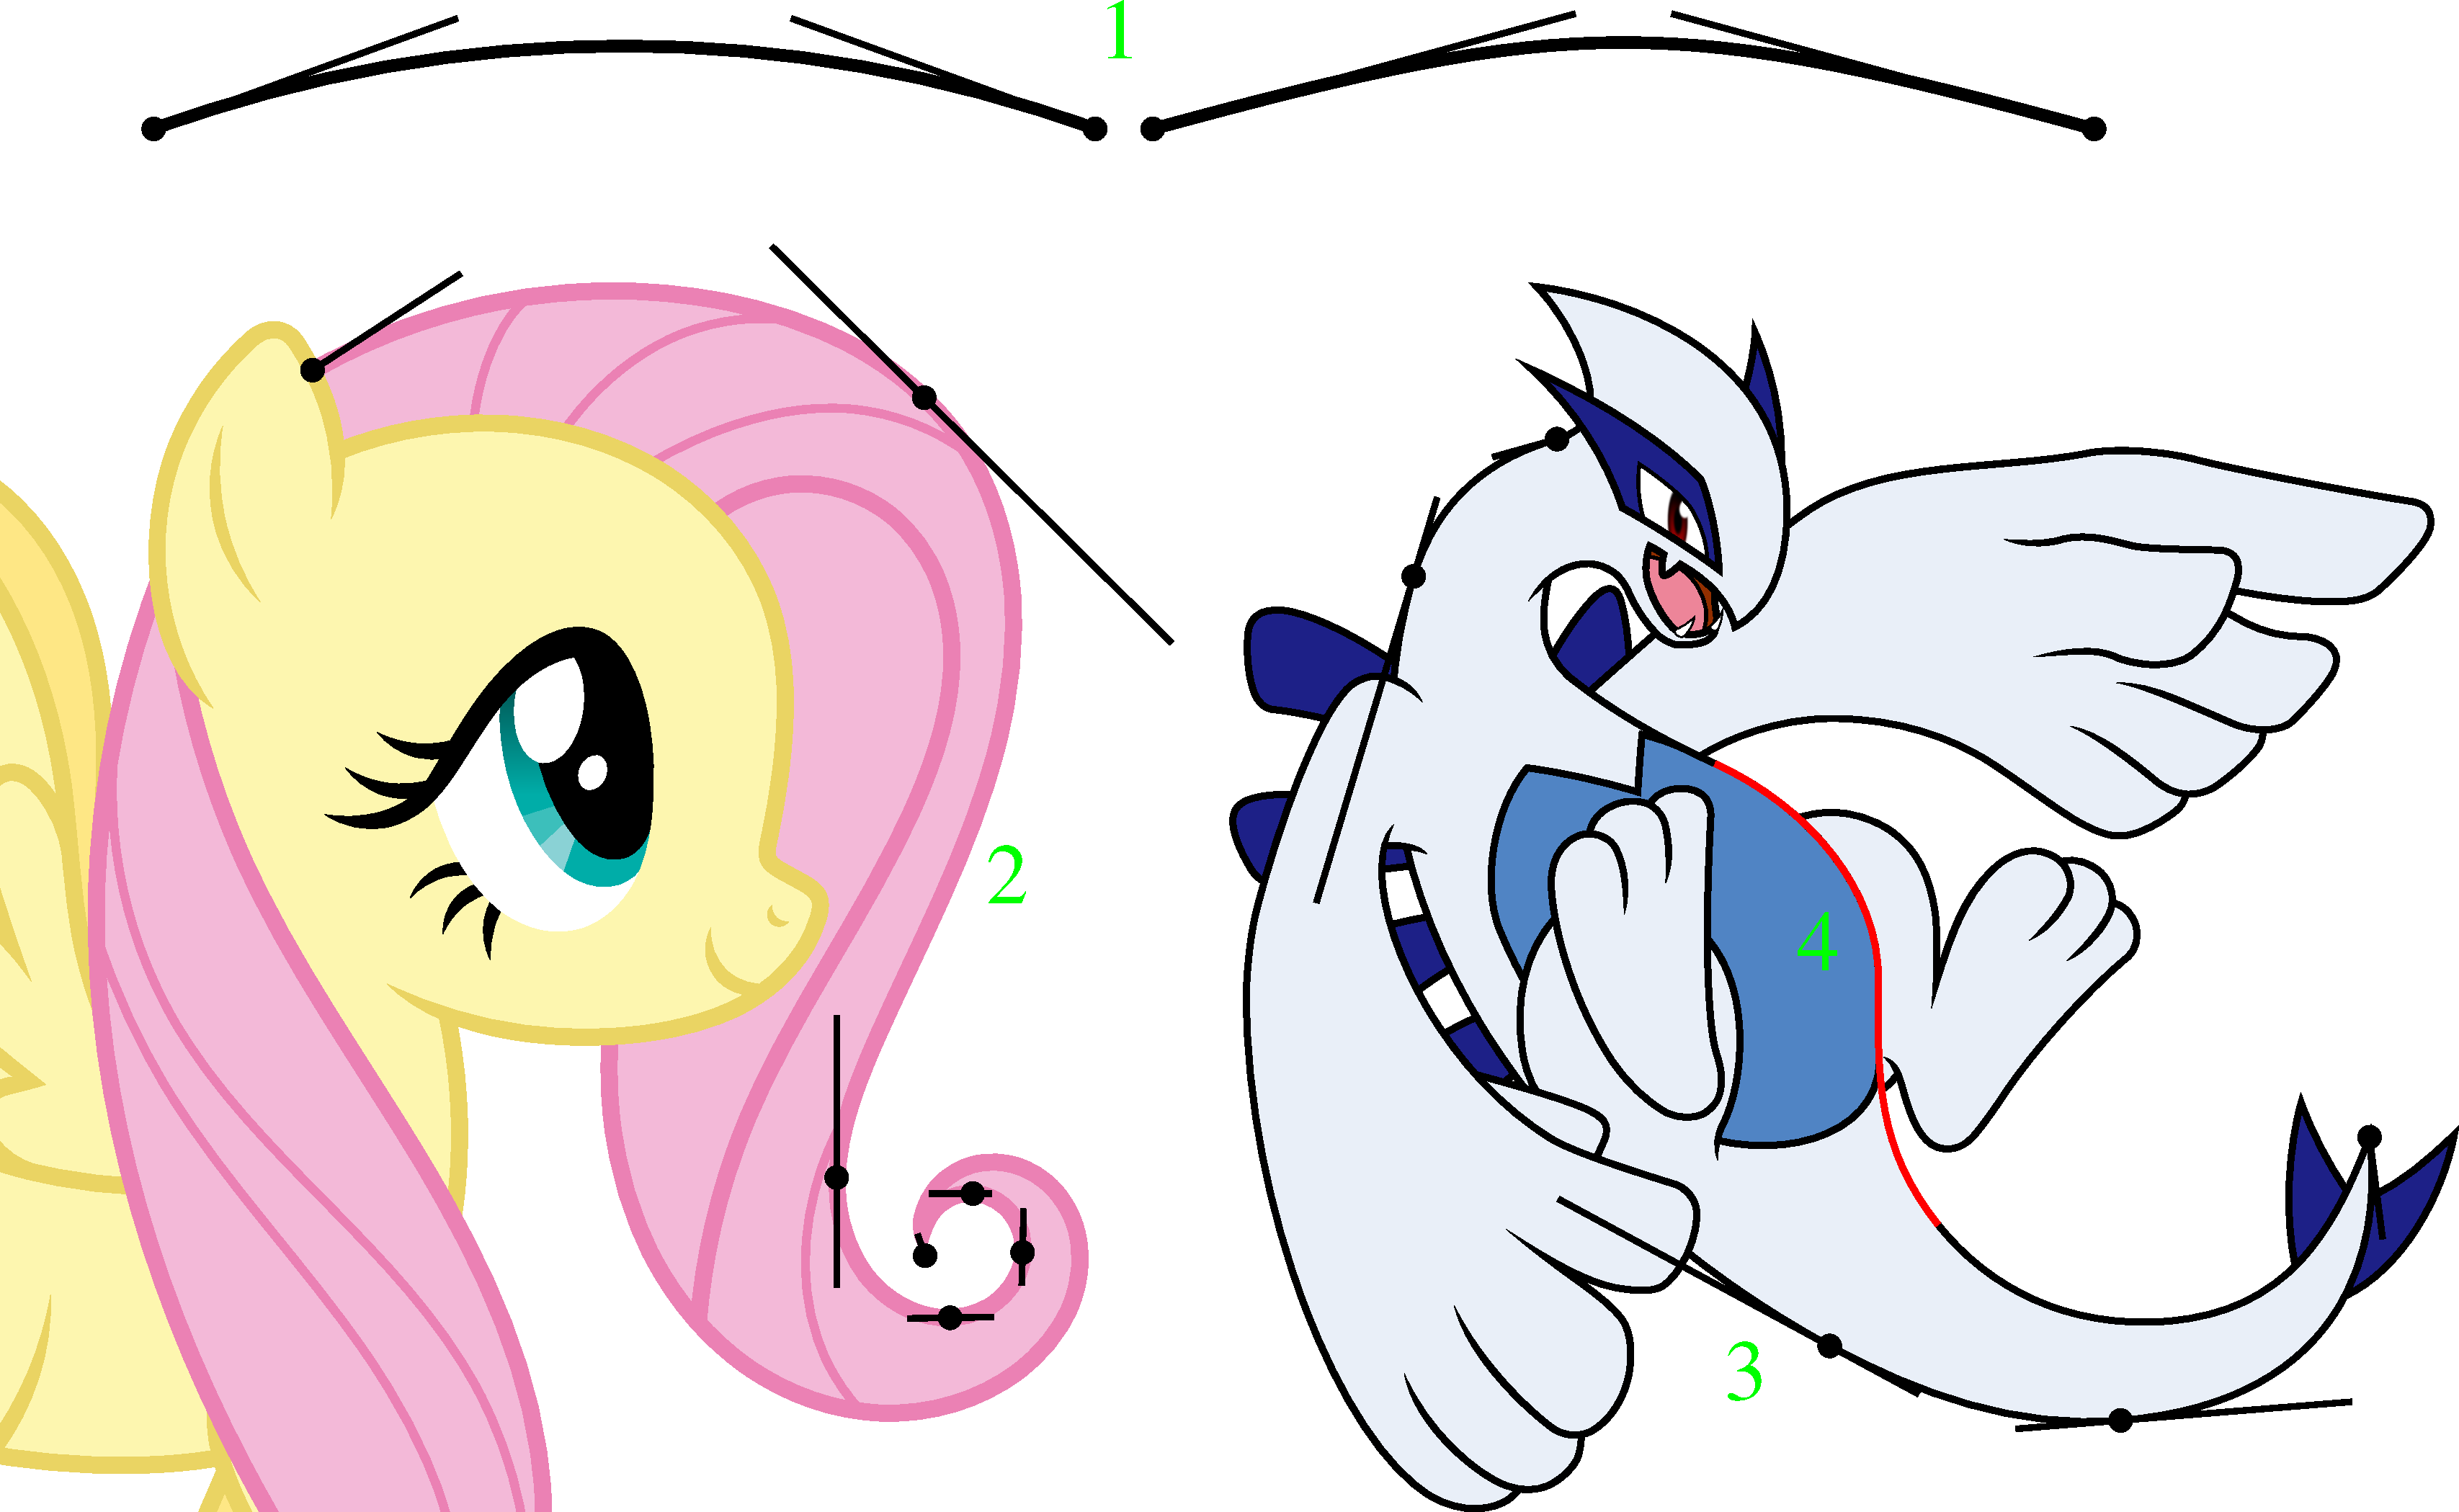
\includegraphics[width=\textwidth]{../resources/usability_bezier.pdf}\\
			\end{centering}
		\end{frame}
		
		\begin{frame}
			\frametitle{Spiro Splines}
			\begin{itemize}
				\item constructed from segments of the Euler spiral
				\item can only specify points (no direction or curvature)
				\item guarantees curvature continuity
				\item only major problem is insufficient expressiveness of specification language
			\end{itemize}
		\end{frame}
		
		\begin{frame}
			\frametitle{Usability Analysis of Spiro Splines}
			\begin{centering}
				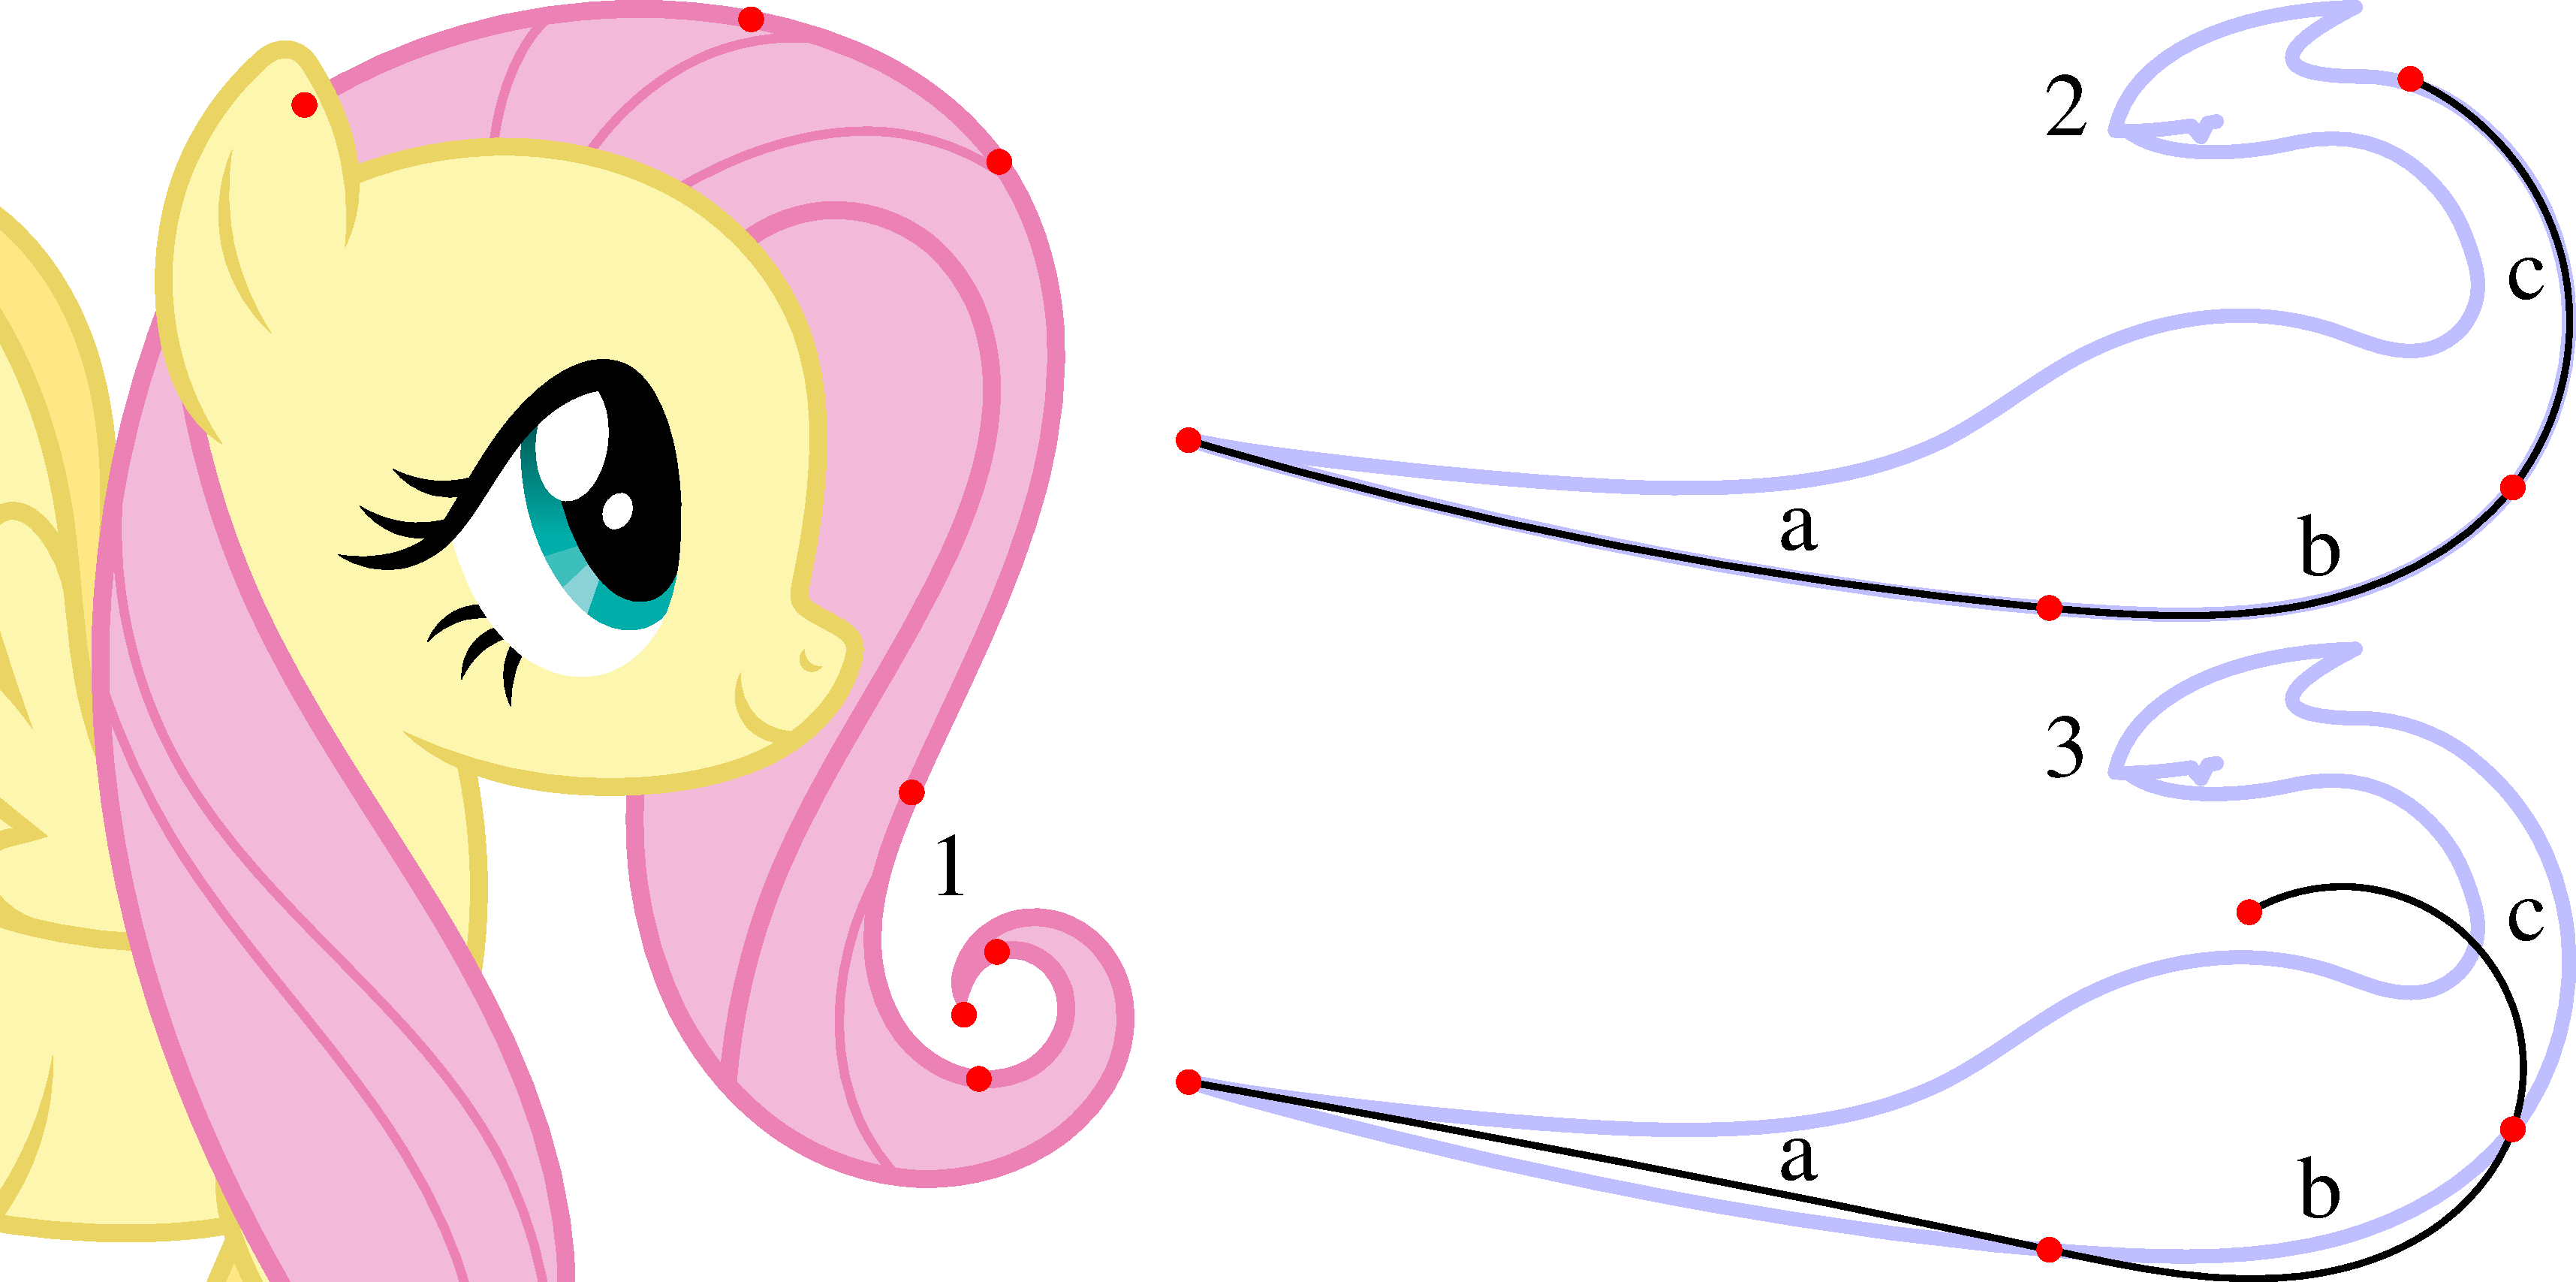
\includegraphics[width=\textwidth]{../resources/usability_spiro.pdf}\\
			\end{centering}
		\end{frame}
	
	\section{Proposed Solution}
	
		\begin{frame}
			\frametitle{Description-Based Curves}
			\begin{itemize}
				\item description language has huge effect on usability
				\item we need a good specification language and fairness measure
			\end{itemize}
		\end{frame}
	
		\begin{frame}
			\frametitle{Description-Based Curves}
			\begin{centering}
				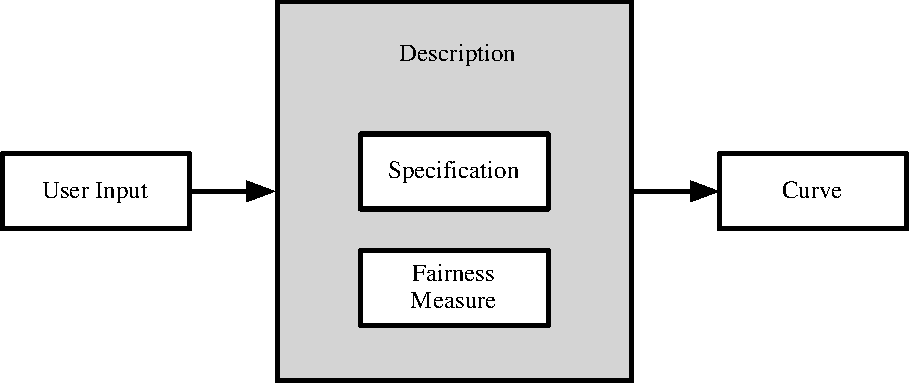
\includegraphics[width=\textwidth]{../resources/description-based_curves.pdf}\\
			\end{centering}
		\end{frame}
		
		\begin{frame}
			\frametitle{Specification Language}
			\begin{itemize}
				\item decoupled from underlying curve model
				\item allows specification of geometric properties
				\item point, direction, curvature
				\item any combination, any position
				\item positioning via fraction of arc length of curve
			\end{itemize}
		\end{frame}

		\begin{frame}
			\frametitle{Specification Language}
			\begin{equation*}
				\begin{alignedat}{2}
					& \mathrm{Positions}          && = \unit\\
					& \mathrm{Points}             && = \R{2}\\
					& \mathrm{Directions}         && = \RR\\
					& \mathrm{Curvatures}         && = \RR\\
					& \mathrm{SpecificationItems} && = \mathrm{Positions} \times \left(\mathrm{Points} \cup \mathrm{Directions} \cup \mathrm{Curvatures}\right)\\
					& \mathrm{CurveLengths}       && = \RR\\
					& \mathrm{Specifications}     && = \powerset{\mathrm{SpecificationItems}} \times \mathrm{CurveLengths}
				\end{alignedat}
			\end{equation*}
		\end{frame}
		
		\begin{frame}
			\frametitle{Fairness Measure}
			\begin{itemize}
				\item chosen fairness measure: minimum variation curves
				\item good at avoiding bumps
			\end{itemize}
			 \begin{equation*}
				 \integral{0}{1}{\apply{\chi'}{t}^2}{t}
			 \end{equation*}
		\end{frame}
		
		\begin{frame}
			\frametitle{Curve Derivation}
			\begin{itemize}
				\item uses nonlinear optimization on polynomial splines
				\item nonlinear optimization: flexible, allows experimentation
				\item polynomial curves: simple yet flexible % through choice of degree
			\end{itemize}
		\end{frame}
		
		\begin{frame}
			\frametitle{Optimization Problem}
			\begin{itemize}
				\item expressed using:
				\begin{itemize}
					\item objective function \(f : \function{\R{n}}{\RR}\)
					\item constraint function \(g : \function{\R{n}}{\R{m}}\)
					\item constraint bounds \(g_l, g_u \in \R{m}\)
				\end{itemize} 
				\item tries to find an \(x^* \in \R{n}\) such that 
			\end{itemize}
			\begin{equation*}
				\begin{gathered}
					x^* = \argmin_{x \in \R{n}} \apply{f}{x}\\
					g_l \leq \apply{g}{x^*} \leq g_u
				\end{gathered}
			\end{equation*}
		\end{frame}
		
		
		\begin{frame}
			\frametitle{Segmentation}
			\begin{itemize}
				\item polynomial spline is determined by the coefficients of each polynomial segment
				\item all coefficients are the optimization domain
				\item segments laid out consecutively with equal length
			\end{itemize}
		\end{frame}
		
		\begin{frame}
			\frametitle{}
			\begin{itemize}
			\end{itemize}
		\end{frame}
		
\end{document}
